\section{Code}
All code I used for this project is publicly accessible at \url{https://github.com/ancuongnguyen07/CS-C320-ML/blob/master/code/notebook.ipynb}

\section{Tables of features}
\begin{table}
    \centering
    \begin{tabular}{|c|c|c|}
        \hline
         & Feature & Value Type \\
        \hline
        1 & NumDots & Int \\
        \hline
        2 & SubdomainLevel & Int \\
        \hline
        3 & PathLevel & Int \\
        \hline
        4 & UrlLength & Int \\
        \hline
        5 & NumDash & Int \\
        \hline
        6 & NumDashInHostName & Int \\
        \hline
        7 & AtSymbol & Int \\
        \hline
        $\cdots$ & $\cdots$ & $\cdots$ \\
        \hline
        47 & ExtMetaScriptLinkRT & Int \\
        \hline
        48 & PctExtNullSelfRedirectHyperlinksRT & Int \\
        \hline
    \end{tabular}
    \caption{Table of all features in the dataset.}\label{tab:all_features}
\end{table}


\begin{longtable}{|c|p{0.15\linewidth}|p{0.4\linewidth}|c|c|}
    \hline
     & Feature & Description & Value Type & Baseline \\
    \hline
    1 & {\hspace{0pt}} FrequentDomainNameMismatch & If the most frequent domain name in HTML source
    code does not match the URL domain name. & Binary (0/1) & Yes\\
    \hline
    2 & {\hspace{0pt}} PathLevel & The depth of the path in URL. & Int & No\\
    \hline
    3 & {\hspace{0pt}} InsecureForms & If the form action attribute contains a URL without HTTPS protocol
    & Binary (1/0) & No\\
    \hline
    4 & {\hspace{0pt}} UrlLength & The total characters in the URL. & Int & No\\
    \hline
    5 & {\hspace{0pt}} PctExtNullSelfRedirectHyperlinksRT & The percentage of hyperlinks in HTML source
    code that uses different domain names, starts with “\#”, or using “JavaScript ::void(0)”.
    \begin{itemize}
        \item request URL\% $<$ 20\% $\rightarrow$ -1: low risk
        \item 20\% $\leq$ request URL\% $<$ 50\% $\rightarrow$ 0: suspecious
        \item otherwise $\rightarrow$ 1: high risk
    \end{itemize} & Categorical & Yes\\
    \hline
    6 & {\hspace{0pt}} NumDash & The number of ``-'' in URL. & Int & Yes\\
    \hline
    7 & {\hspace{0pt}} QueryLength & The total characters in query part of URL. & Int & No\\
    \hline
    8 & {\hspace{0pt}} SubmitInfoToEmail & If HTML source code contains the HTML ``mailto'' function.
    & Binary (0/1) & Yes\\
    \hline
    9 & {\hspace{0pt}} NumNumericChars & The number of numeric characters in URL. & Int & Yes\\
    \hline
    10 & {\hspace{0pt}} NumDots & The number of dots in URL & Int & No\\
    \hline
    11 & {\hspace{0pt}} PathLength & The total characters in path of URL. & Int & No\\
    \hline
    12 & {\hspace{0pt}} PctExtResourceUrlsRT& The percentage of external resource URLs in HTML source
    code. Applied threshold rules.
    \begin{itemize}
        \item request URL\% $<$ 20\% $\rightarrow$ -1: Legitimate
        \item 20\% $\leq$ request URL\% $<$ 50\% $\rightarrow$ 0: Suspecious
        \item otherwise $\rightarrow$ 1: Phishy
    \end{itemize}
    & {\hspace{0pt}} Categorical & Yes\\
    \hline
    13 & {\hspace{0pt}} PctNullSelfRedirectHyperlinks & The percentage of hyperlinks fields containing empty
    value, self-redirect value such as ``\#'', URL of current webpage, or some abnormal value such as
    ``file://E:/'' & Float & Yes\\
    \hline
    14 & {\hspace{0pt}} NumSensitiveWords & The number of sensitive words (i.e., “secure”, “account”, “webscr”,
    “login”, “ebayisapi”, “signin”, “banking”, “confirm”) in webpage URL & Int & Yes\\
    \hline
    15 & {\hspace{0pt}} PctExtHyperlinks & The percentage of external hyperlinks in webpage HTML source code
    & Float & Yes\\
    \hline
    16 & {\hspace{0pt}} ExtMetaScriptLinkRT & The percentage of meta, script and link tags containing external
    URL in the attributes. Applied threshold rules.
    \begin{itemize}
        \item external URL\% $<$ 20\% $\rightarrow$ -1: Legitimate
        \item 20\% $\leq$ external URL\% $<$ 50\% $\rightarrow$ 0: Suspecious
        \item otherwise $\rightarrow$ 1: Phishy
    \end{itemize} & Categorical & Yes\\
    \hline
    \caption{Feature Description and Value Types.}\label{tab:feature_description}
\end{longtable}

\section{Feature Statistic}
\begin{figure}[ht!]
    \centering
    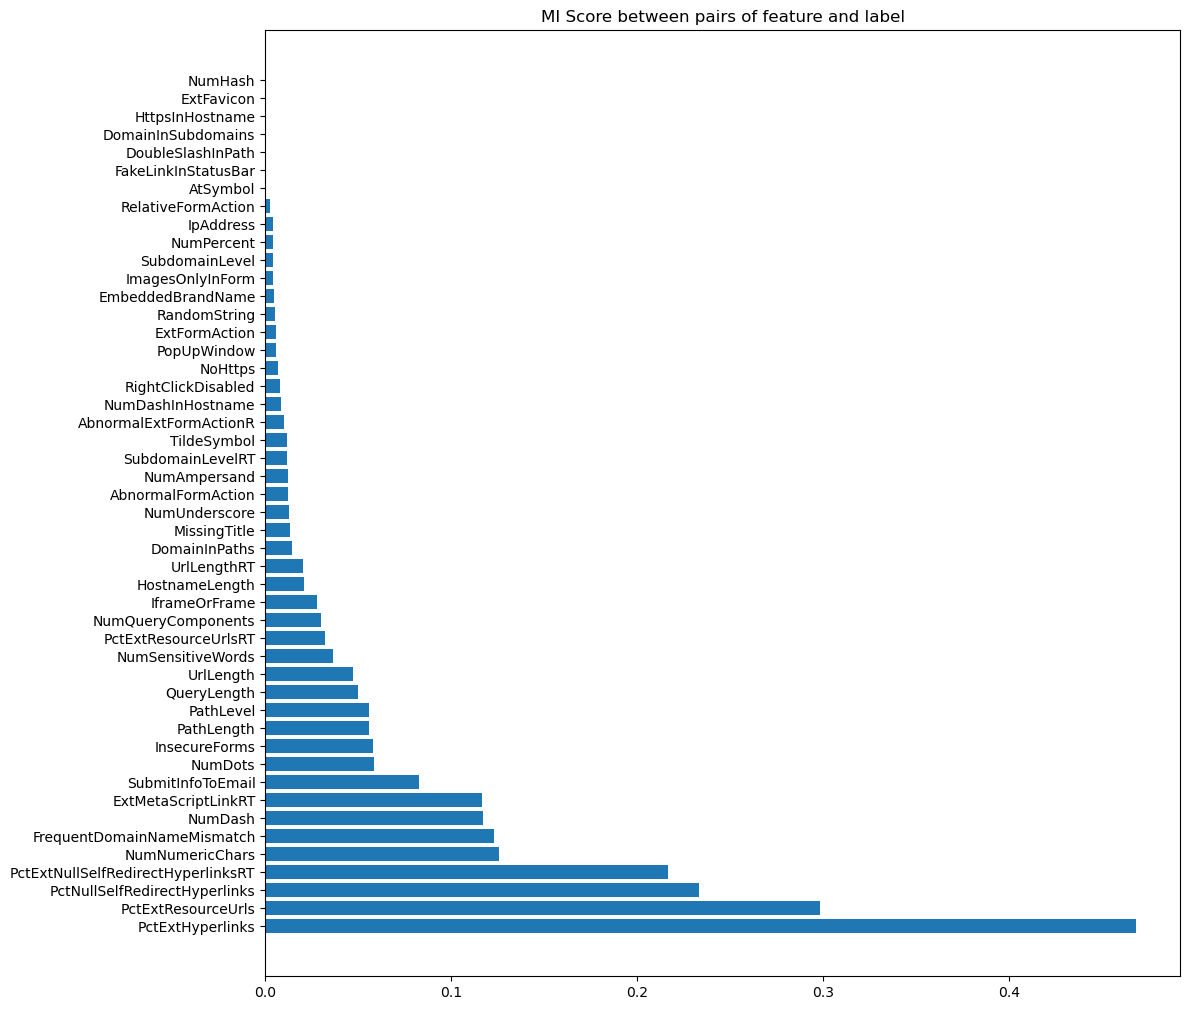
\includegraphics[width=\textwidth,height=\textheight,keepaspectratio,scale=1.5]
    {MI_score.png}
    \caption{Mutual Information (MI) Scores of all features}\label{fig:mi_score}
\end{figure}

\begin{figure}
    \centering
    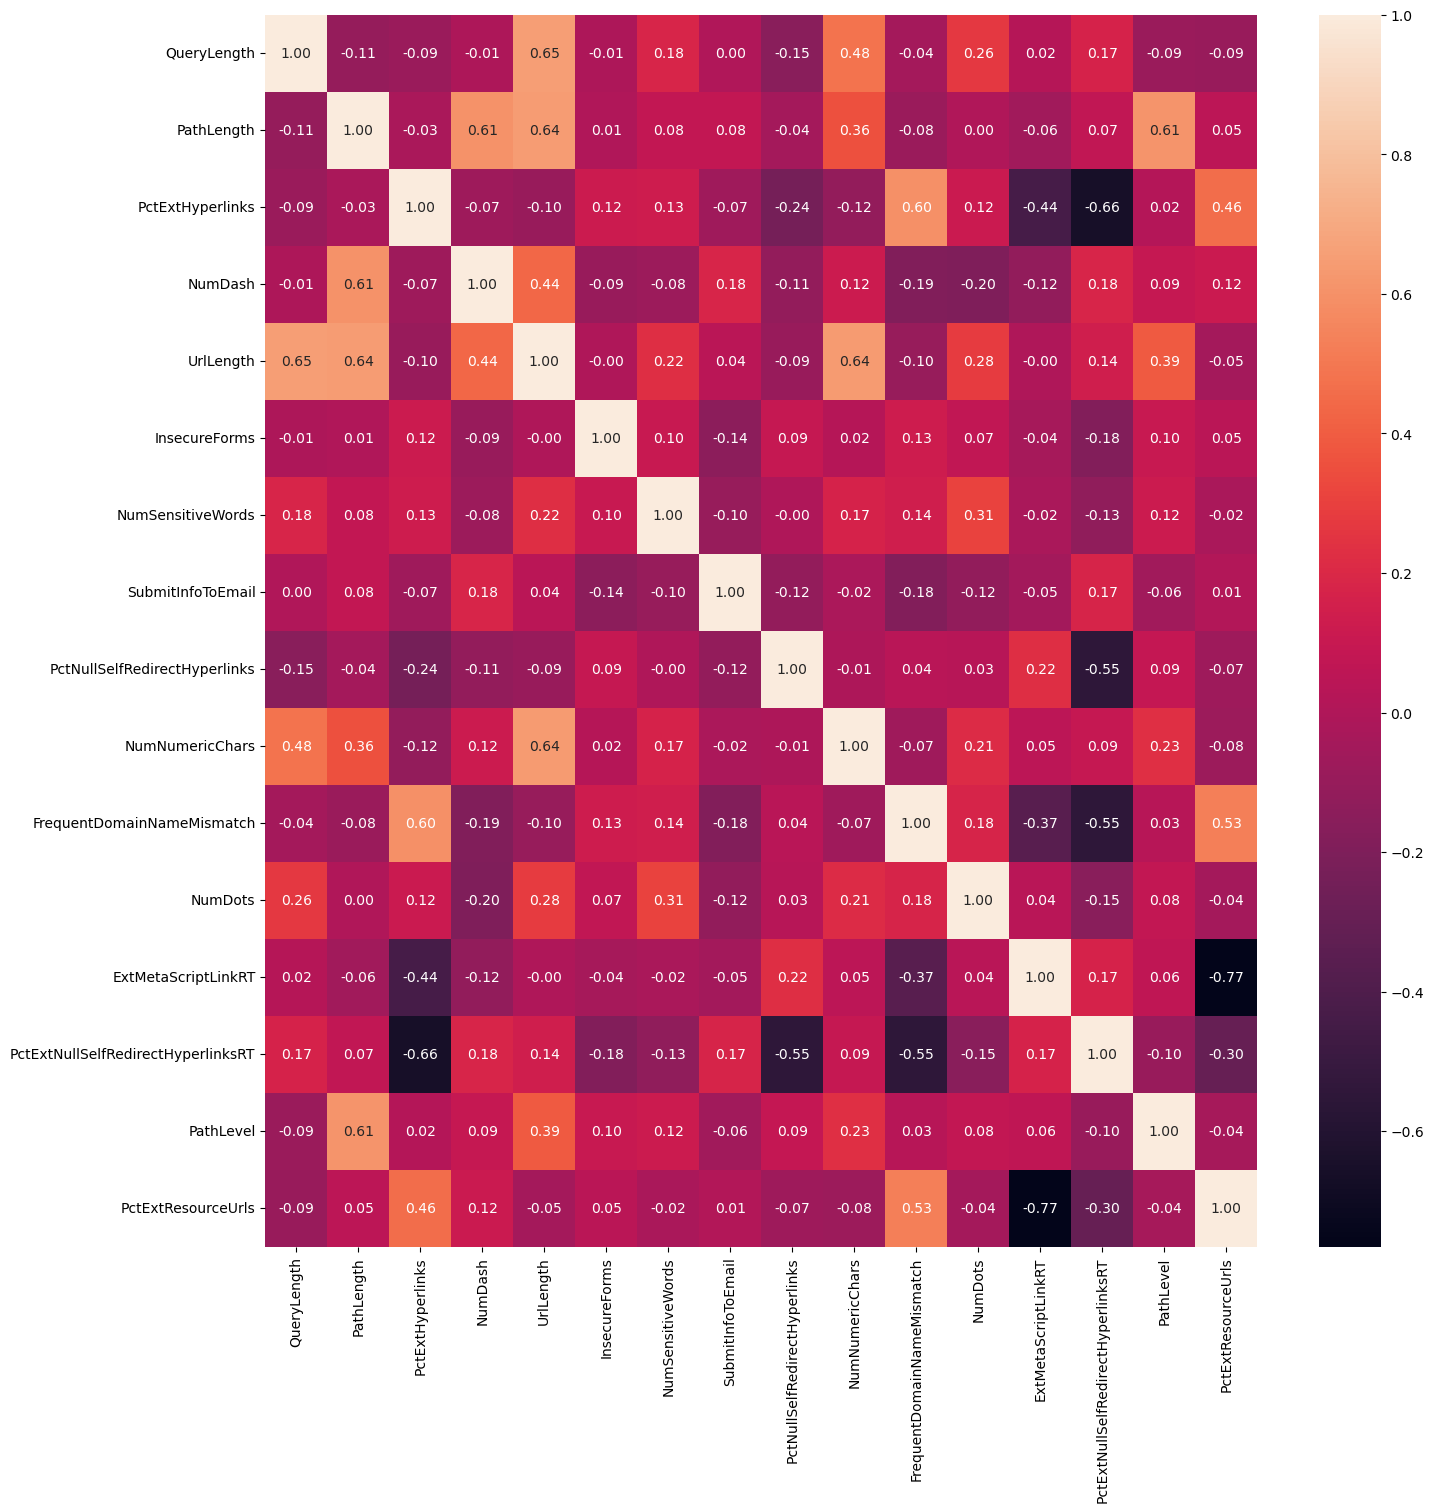
\includegraphics[width=\textwidth,height=\textheight,keepaspectratio]
    {feature-linear-relation.png}
    \caption{Pairwise correlation between features in the custom set.}
    \label{fig:feature-correlation}
\end{figure}

\section{Confusion Matrices}
\begin{figure}[ht!]
    \centering
    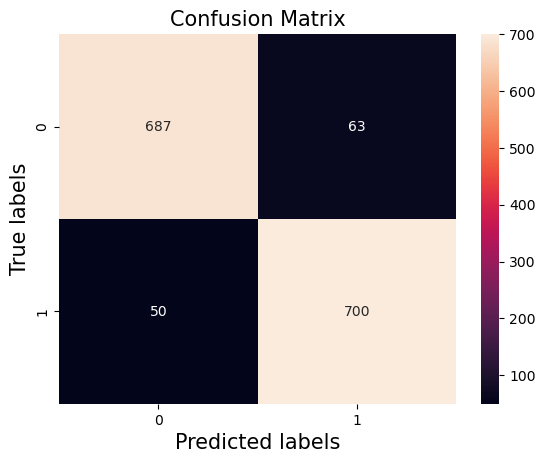
\includegraphics[width=\textwidth,height=\textheight,keepaspectratio]
    {conf-mat-lr-val.png}
    \caption{Confusion Matrix generated by the LR model on the validation set.}
    \label{fig:conf-mat-lr-val}
\end{figure}

\begin{figure}[ht!]
    \centering
    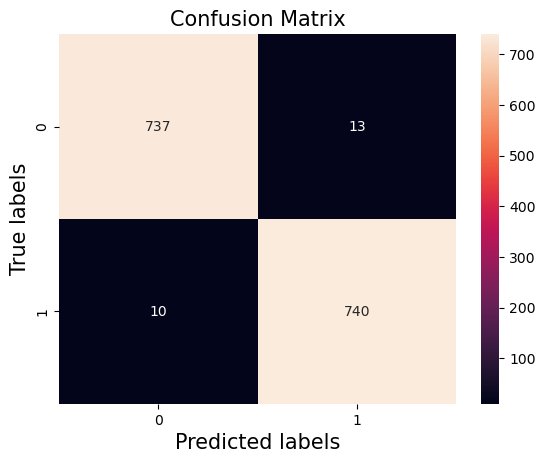
\includegraphics[width=\textwidth,height=\textheight,keepaspectratio]
    {conf-mat-rf-val.png}
    \caption{Confusion Matrix generated by the RF model on the validation set.}
    \label{fig:conf-mat-rf-val}
\end{figure}

\begin{figure}[ht!]
    \centering
    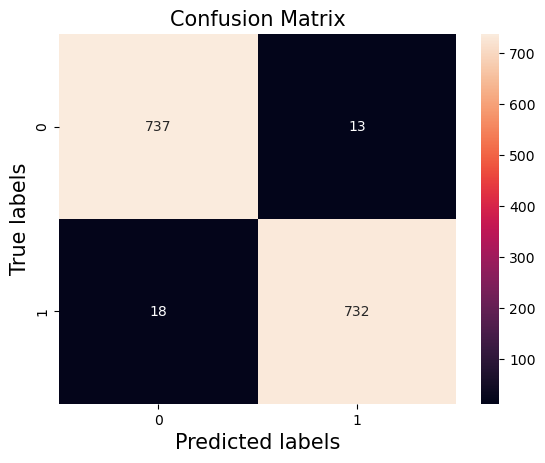
\includegraphics[width=\textwidth,height=\textheight,keepaspectratio]
    {conf-mat-rf-test.png}
    \caption{Confusion Matrix generated by the RF model on the test set.}
    \label{fig:conf-mat-rf-test}
\end{figure}

\begin{figure}
    \centering
    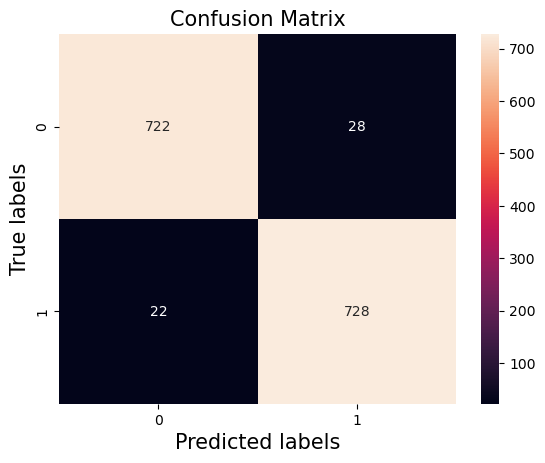
\includegraphics[width=\textwidth,height=\textheight,keepaspectratio]
    {conf-mat-rf-baseline-test.png}
    \caption{Confusion Matrix generated by the RF model (baseline features) on the test set.}
    \label{fig:conf-mat-rf-baseline-test}
\end{figure}
